\begin{chapter}{Applications and Numerical Experiments}
\label{ch:numericalexperiments}

\section{Image denoising} % (fold)
\label{sec:image denoising}
The very basic application of the algorithm is of course denoising of common 2D grayscale or color pictures.
For grayscale pictures the TV minimization is performed over the Euclidian manifold $M=\mathbb{R}$, while for color
picture, as already explained in the introduction, we have either $M=\mathbb{R}^3$ for the linear-vectorial model or
$M=S^2\times\mathbb{R}$ for the non-linear chromaticity-brightness model.

\subsection{Grayscale} % (fold)
\label{sub:Grayscale}
% subsection Grayscale (end)

\FloatBarrier
\subsection{Color} % (fold)
\label{sub:Color}
In this example we perform the TV minimization of color images using the two different color models. In Figure \ref{fig:application_color1}
the among the image processing community well-known \emph{Lena} picture which is 


% subsection Color (end)
\begin{figure}[h!]
    \centering
    \subfloat[][Original]{
	\label{fig:application_color1_orig}
	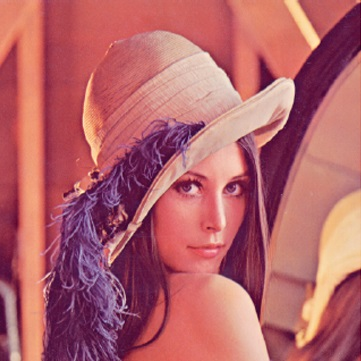
\includegraphics[width=0.325\linewidth]{./figures/experiments/Lena.jpg}
    }
    \subfloat[][Noised]{
	\label{fig:application_color1_noise}
	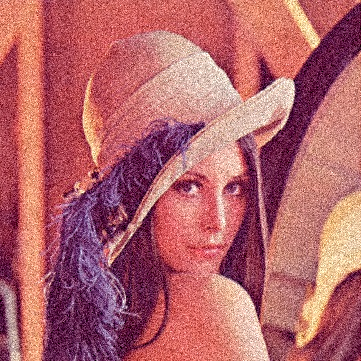
\includegraphics[width=0.325\linewidth]{./figures/experiments/Lena_noise.jpg}
    }
    \subfloat[][Denoised]{
	\label{fig:application_color1_denoised}
	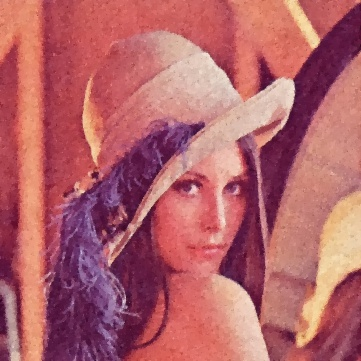
\includegraphics[width=0.325\linewidth]{./figures/experiments/denoised_Lena_noise.jpg}
    }\\
    \caption[Denoising linear vectorial]{Denoising of a color images using the linear vectorial color model which corresponds to the manifold $\mathbb{R}^3$
	\subref{fig:application_color1_orig} Original image "Lena.jpg", $361\times 361$ px, 8 bit color depth
	\subref{fig:application_color1_noise} Componentwise gaussian noise $\mu=0$, $\sigma=?$ added
	\subref{fig:application_color1_denoised} Denoised, IRLS with $\lambda=?$, $?$ IRLS steps, $?$ newton steps per IRLS step
	\label{fig:application_color1}
    }
\end{figure}

\begin{figure}[h!]
    \centering
    \subfloat[][Original]{
	\label{fig:application_color2_orig}
	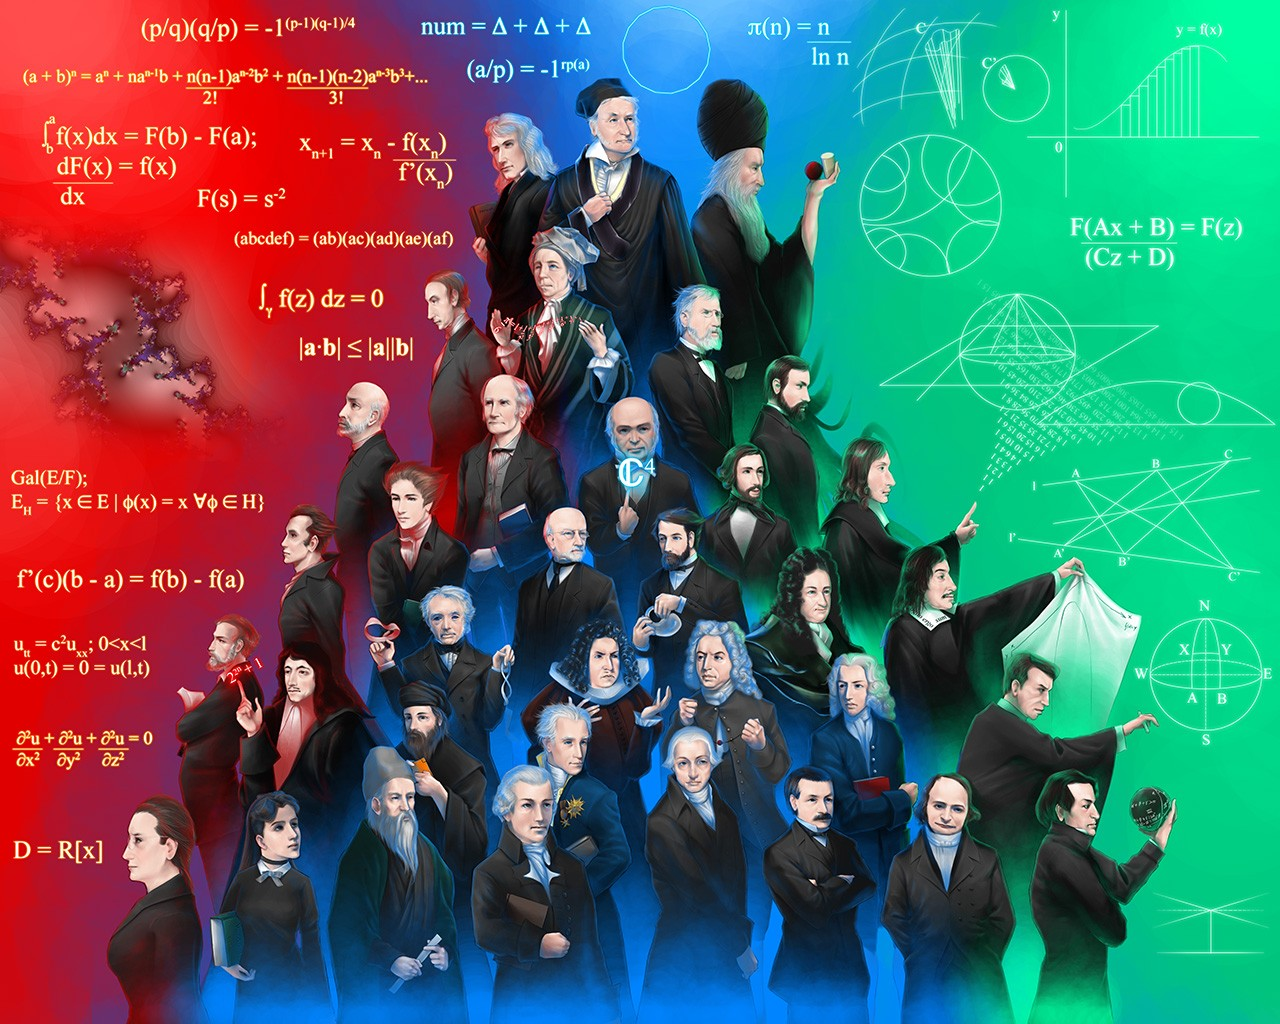
\includegraphics[width=0.325\linewidth]{./figures/experiments/mathematicians.jpg}
    }
    \subfloat[][Noised]{
	\label{fig:application_color2_noise}
	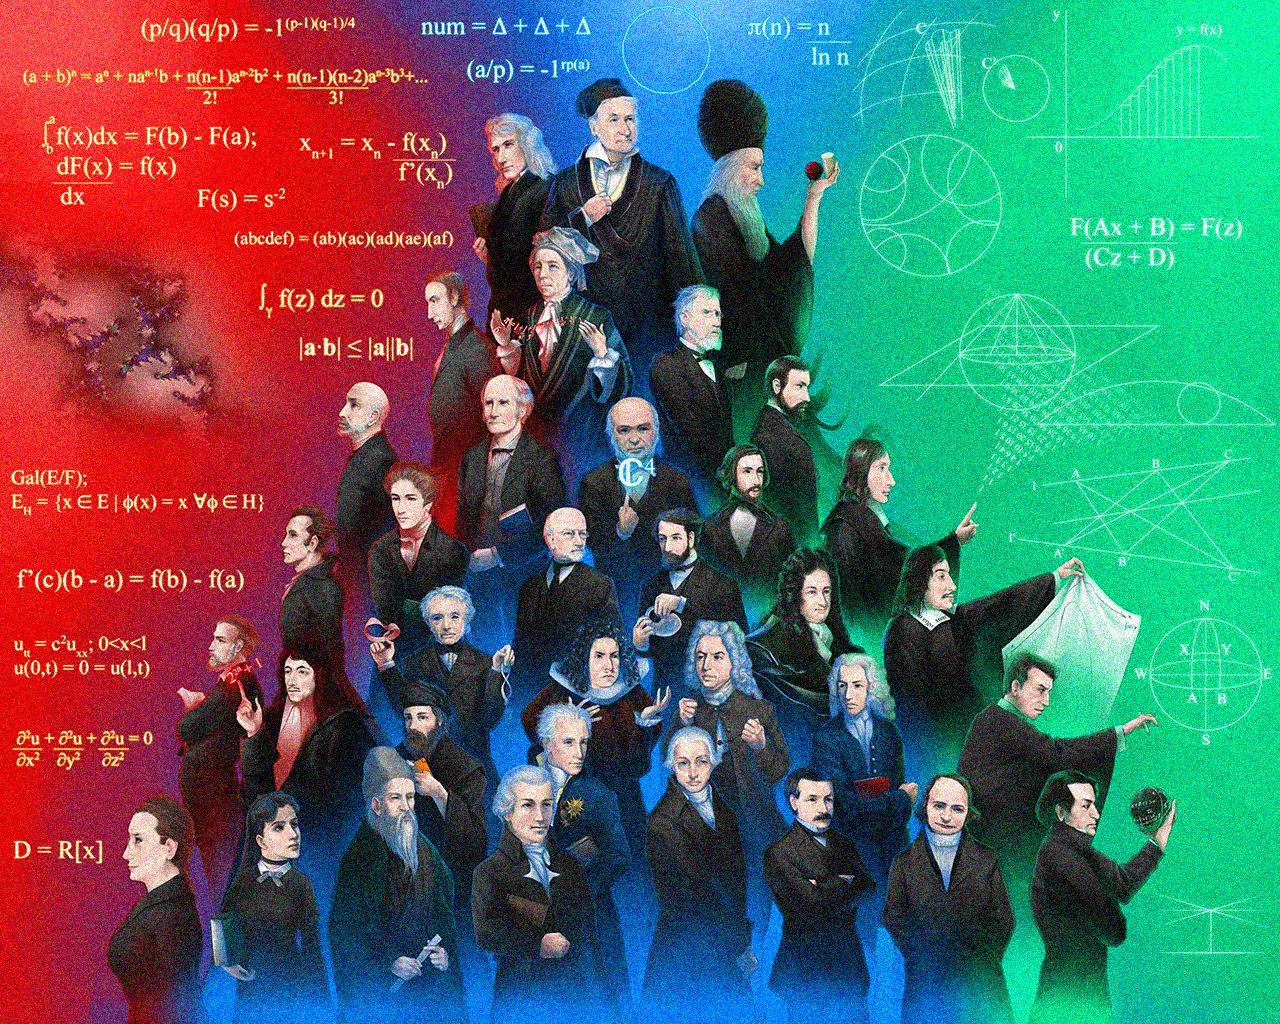
\includegraphics[width=0.325\linewidth]{./figures/experiments/noisy_mathematicians.jpg}
    }
    \subfloat[][Denoised]{
	\label{fig:application_color2_denoised}
	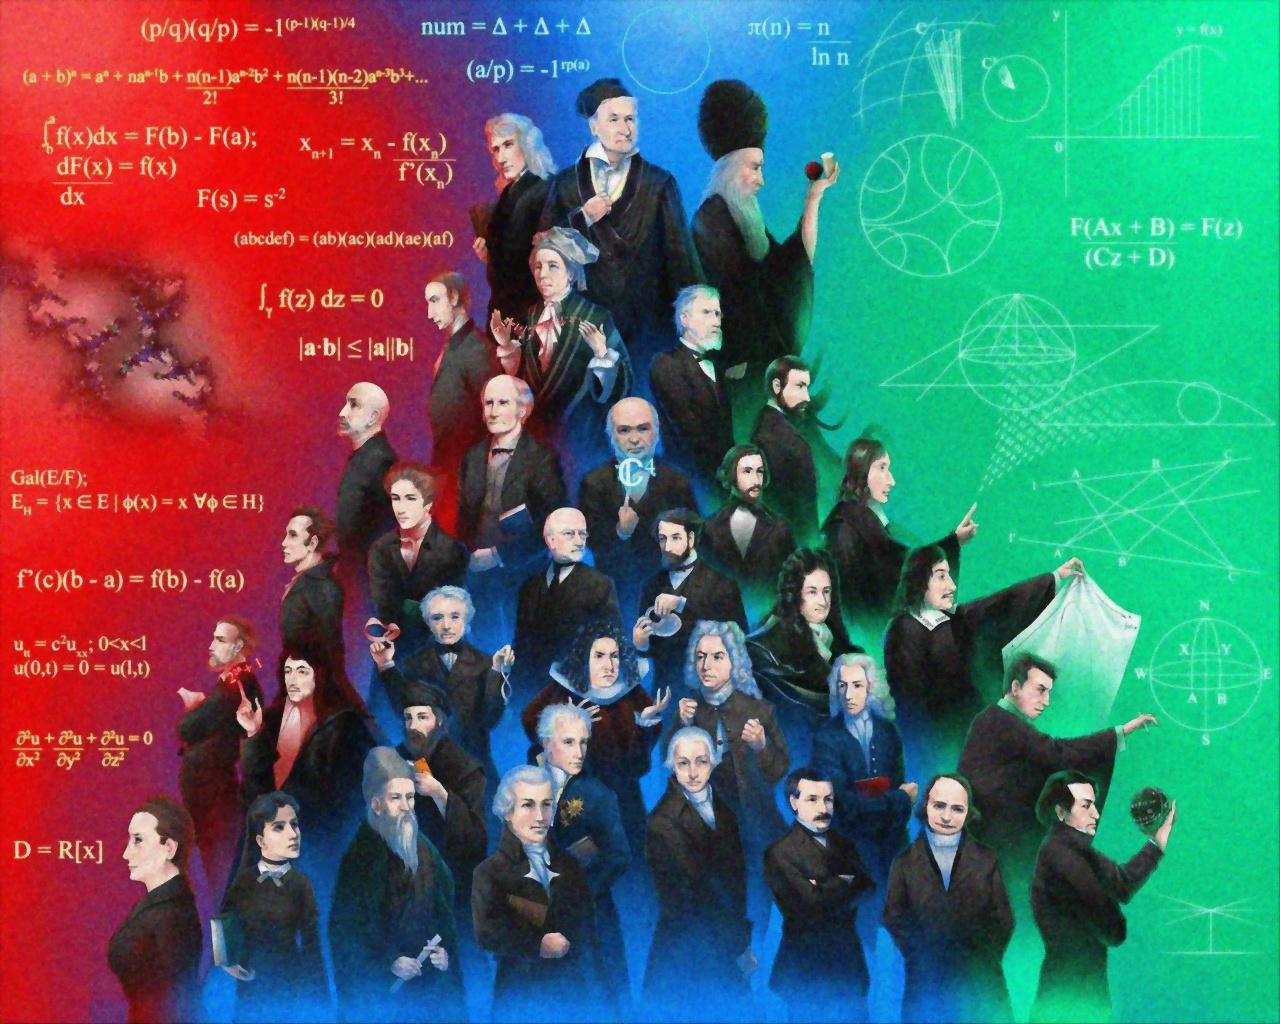
\includegraphics[width=0.325\linewidth]{./figures/experiments/denoised_noisy_mathematicians.jpg}
    }\\
    \caption[Denoising linear vectorial]{Denoising of a color images using the linear vectorial color model which corresponds to the manifold $\mathbb{R}^3$
	\subref{fig:application_color2_orig} Original image "mathematicians.jpg", $1280\times 1024$ px, 8 bit color depth
	\subref{fig:application_color2_noise} Componentwise gaussian noise $\mu=0$, $\sigma=?$ added
	\subref{fig:application_color2_denoised} Denoised, IRLS with $\lambda=?$, $?$ IRLS steps, $?$ newton steps per IRLS step
	\label{fig:application_color2}
    }
\end{figure}


\FloatBarrier
\subsection{Inpainting} % (fold)
\label{sub:Inpainting}
\begin{figure}[h!]
    \centering
    \subfloat[][Original]{
	\label{fig:application_colorinpaint1_orig}
	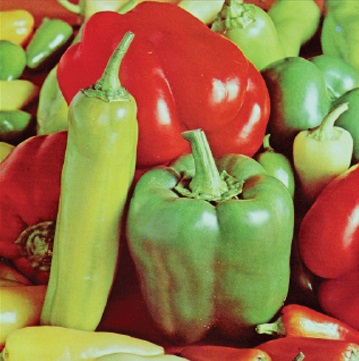
\includegraphics[width=0.25\linewidth]{./figures/experiments/Pepper.jpg}
    }
    \subfloat[][Damaged]{
	\label{fig:application_colorinpaint1_dam}
	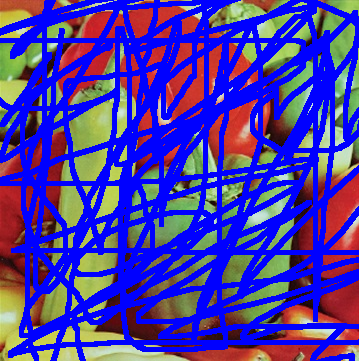
\includegraphics[width=0.25\linewidth]{./figures/experiments/Pepper_dam.png}
    }
    \subfloat[][First guess]{
	\label{fig:application_colorinpaint1_guess}
	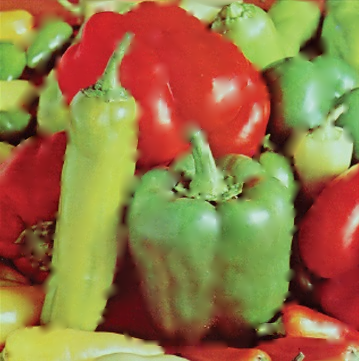
\includegraphics[width=0.25\linewidth]{./figures/experiments/firstguess_Pepper_dam.png}
    }
    \subfloat[][Restored]{
	\label{fig:application_colorinpaint1_restored}
	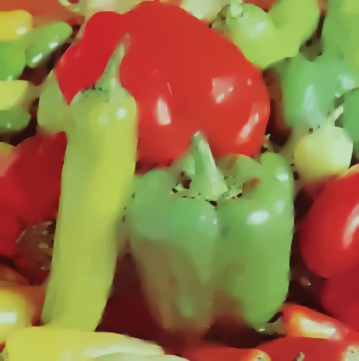
\includegraphics[width=0.25\linewidth]{./figures/experiments/denoised_Pepper_dam.png}
    }\\
    \caption[Denoising linear vectorial]{Denoising of a color images using the linear vectorial color model which corresponds to the manifold $\mathbb{R}^3$
	\subref{fig:application_colorinpaint1_orig} Original image "Pepper.png", $359\times 361$ px, 8 bit color depth
	\subref{fig:application_colorinpaint1_dam} Damaged by overpainting with blue color
	\subref{fig:application_colorinpaint1_guess} First guess via componentwise scattered interpolation
	\subref{fig:application_colorinpaint1_restored} Restored, IRLS with $\lambda=?$, $?$ IRLS steps, $?$ newton steps per IRLS step
	\label{fig:application_colorinpaint1}
    }
\end{figure}

% subsection Inpainting (end)


\FloatBarrier
\subsection{Recolorization} % (fold)
\label{sub:Recolorization}
\begin{figure}[h!]
    \centering
    \subfloat[][Original]{
	\label{fig:application_colorization1_orig}
	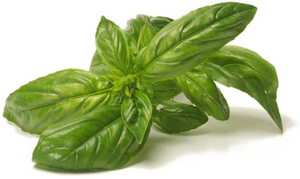
\includegraphics[width=0.25\linewidth]{./figures/experiments/Basil.jpg}
    }
    \subfloat[][Colors removed]{
	\label{fig:application_colorization1_colorless}
	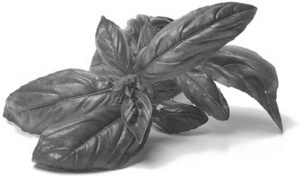
\includegraphics[width=0.25\linewidth]{./figures/experiments/colorless_Basil.jpg}
    }
    \subfloat[][First guess]{
	\label{fig:application_colorization1_guess}
	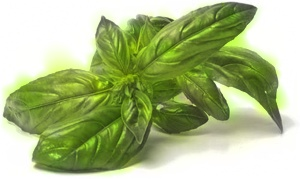
\includegraphics[width=0.25\linewidth]{./figures/experiments/recolored_fg_Basil.jpg}
    }
    \subfloat[][Recolored]{
	\label{fig:application_colorization1_restored}
	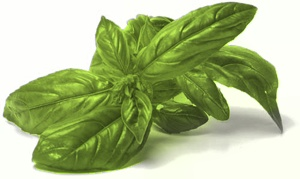
\includegraphics[width=0.25\linewidth]{./figures/experiments/recolored_Basil.jpg}
    }\\
    \caption[Recolorization]{Recolorization using color inpainting in the Chromaticity-Brightness color model, corresponding to $S^2\times\mathbb{R}$
	\subref{fig:application_colorization1_orig} Original image "Basil.jpg", $300\times 179$ px, 8 bit color depth
	\subref{fig:application_colorization1_colorless} Image with a ration of approximately $0.01$ remaining colored pixels
	\subref{fig:application_colorization1_guess} First guess via componentwise scattered interpolation
	\subref{fig:application_colorization1_restored} Recolored, IRLS with $\lambda=?$, $?$ IRLS steps, $?$ newton steps per IRLS step
	\label{fig:application_colorization1}
    }
\end{figure}
% subsection Recolorization (end)

\FloatBarrier
\subsection{Volume images} % (fold)
\label{sub:Volume images}
\begin{figure}[h!]
    \centering
    \subfloat[][Original]{
	\label{fig:application_volume1_orig}
	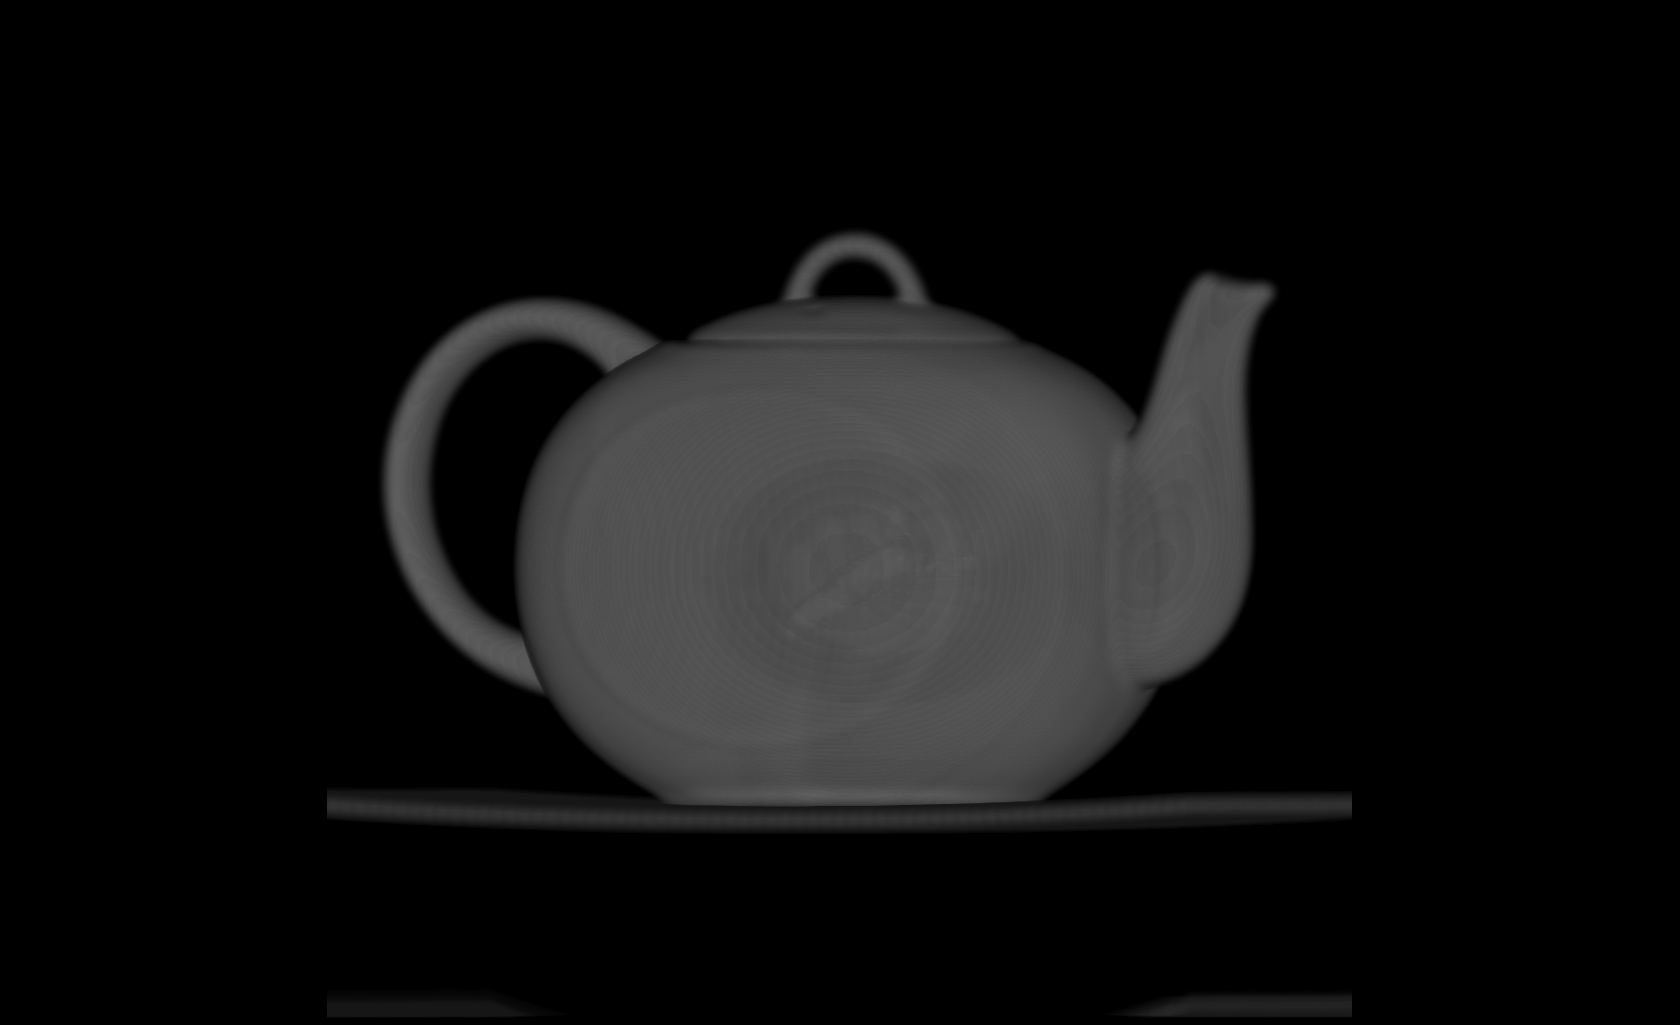
\includegraphics[width=0.325\linewidth]{./figures/experiments/VolumeImg.png}
    }
    \subfloat[][Noised]{
	\label{fig:application_volume1_noise}
	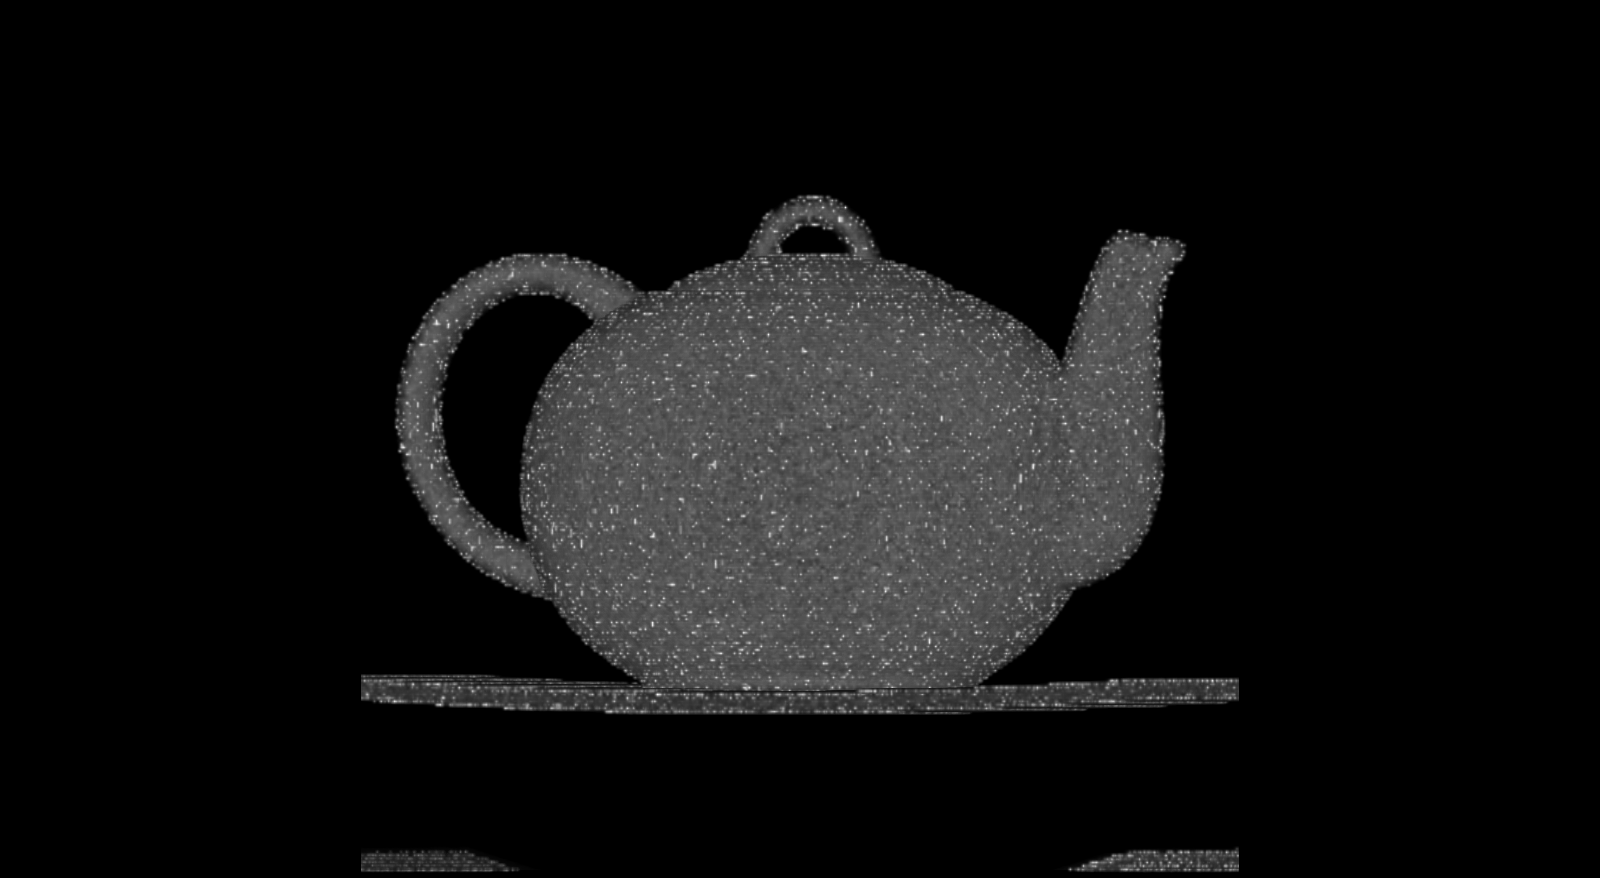
\includegraphics[width=0.325\linewidth]{./figures/experiments/noisyVolumeImg.png}
    }
    \subfloat[][Denoised]{
	\label{fig:application_volume1_denoised}
	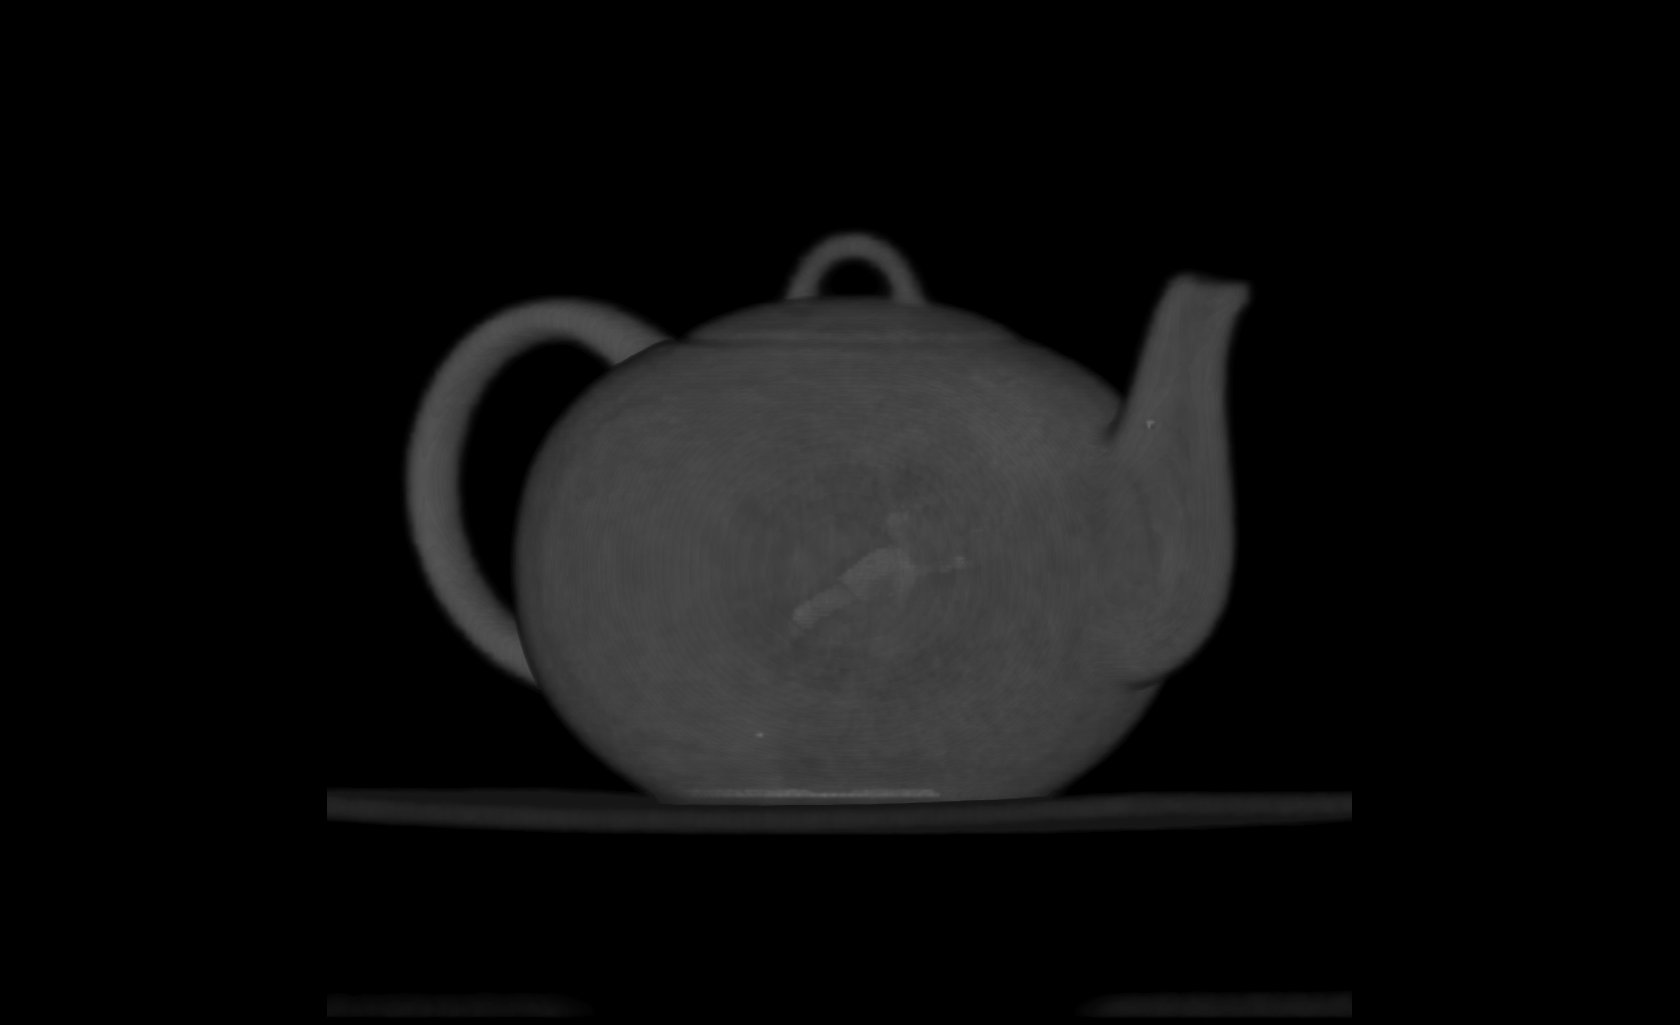
\includegraphics[width=0.325\linewidth]{./figures/experiments/denoisedVolumeImg.png}
    }\\
    \caption[Denoising 3D Grayscale Volume Data]{Denoising a 3D graysclae volume image
	\subref{fig:application_volume1_orig} Original image "BostonTeapot.raw", $256\times 256 \times 178$ px, 8 bit color depth
	\subref{fig:application_volume1_noise} Componentwise gaussian noise $\mu=0$, $\sigma=?$ added
	\subref{fig:application_volume1_denoised} Denoised, Proximal point with $\lambda=?$, $50$ PRPT steps
	\label{fig:application_volume1}
    }
\end{figure}
% subsection Volume images (end)

% section Color image denoising (end)

\FloatBarrier
\section{SO(2) and SO(3) images data} % (fold)
\label{sec:SO images data}

\subsection{Synthetic data} % (fold)
\label{sub:Synthetic data}
\begin{figure}[h!]
    \centering
    \subfloat[][Original]{
	\label{fig:application_so1_orig}
	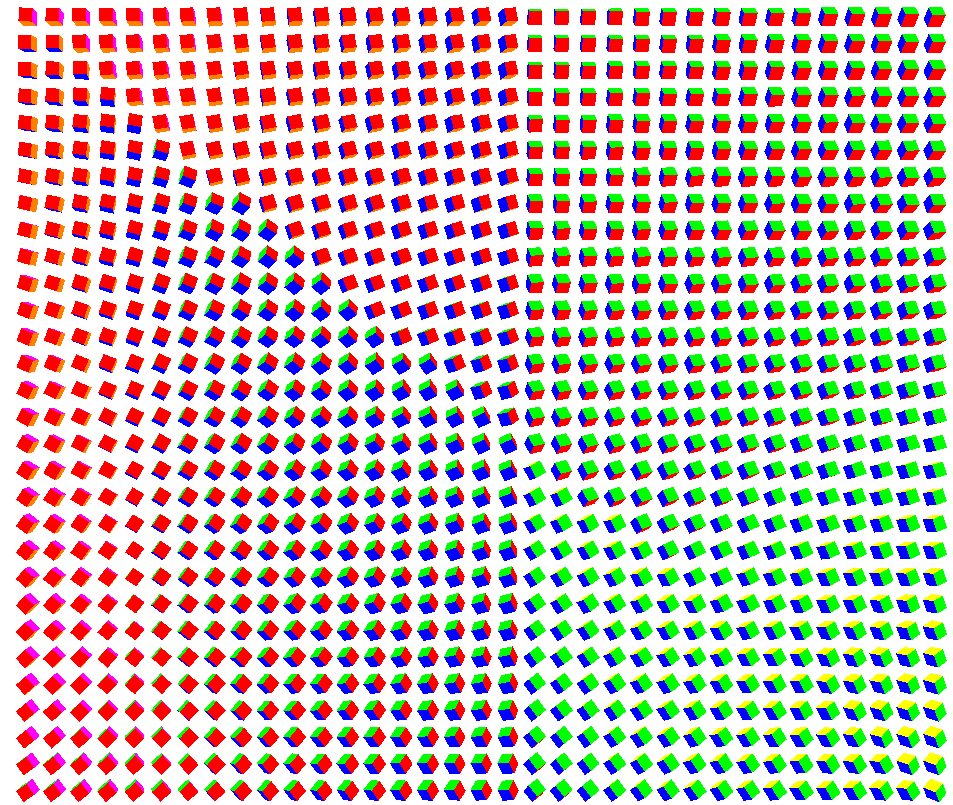
\includegraphics[width=0.325\linewidth]{./figures/experiments/son30x30original.png}
    }
    \subfloat[][Damaged]{
	\label{fig:application_so1_dam}
	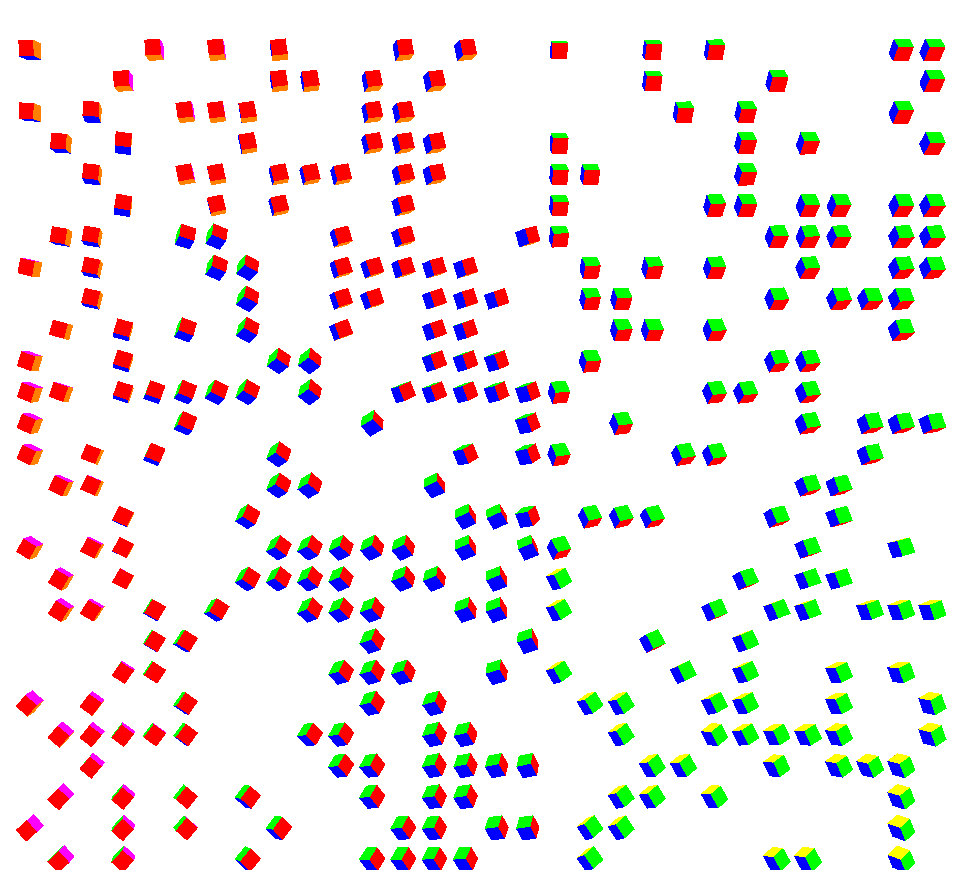
\includegraphics[width=0.325\linewidth]{./figures/experiments/son30x30damaged.png}
    }
    \subfloat[][Reconstructed]{
	\label{fig:application_so1_inp}
	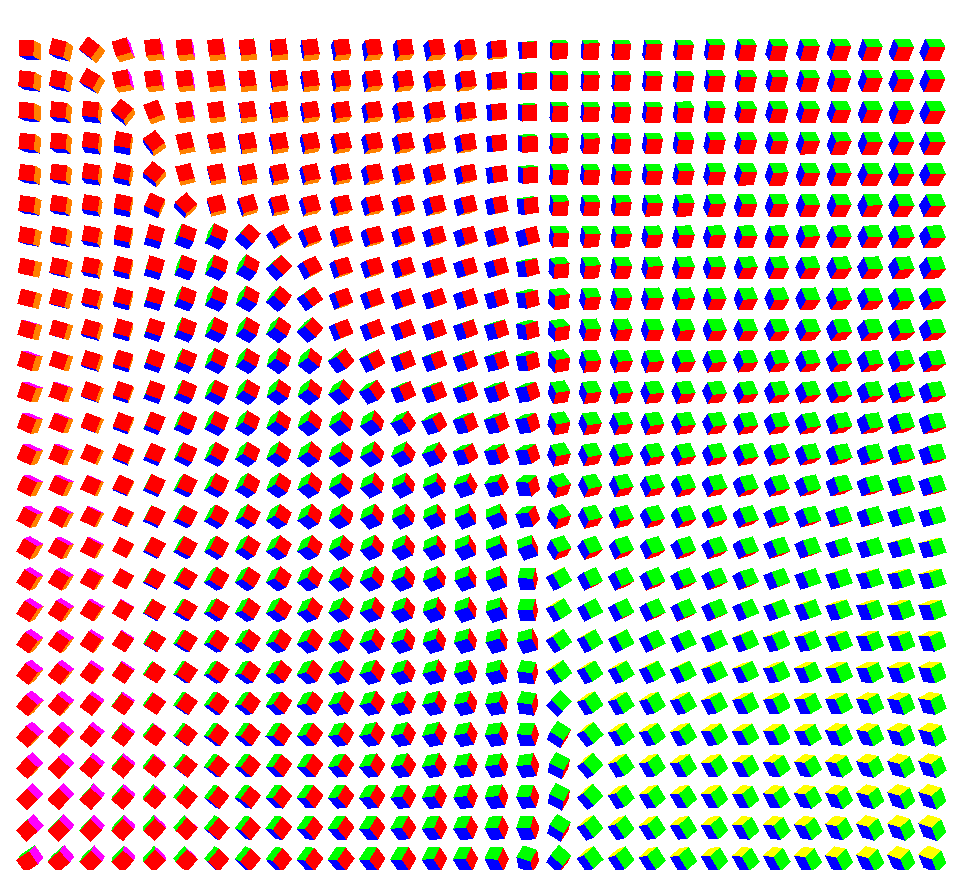
\includegraphics[width=0.325\linewidth]{./figures/experiments/son30x30inpainted.png}
    }\\
    \caption[Inpainting of synthetic SO(3) picture]{Inpainting of synthetic SO(3) picture
	\subref{fig:application_so1_orig} Original image: Synthetic, nonsmooth SO(3), $30\times 30$ px
	\subref{fig:application_so1_dam} Threshold $p=?$
	\subref{fig:application_so1_inp} Denoised, IRLS with $\lambda=?$, 5 IRLS steps, 1 Newton step per IRLS
	\label{fig:application_so1}
    }
\end{figure}

% subsection Synthetic data (end)

\FloatBarrier
\subsection{Fingerprint orientation data} % (fold)
\label{sub:Fingerprint orientation data}
Fingerprint matching is  based on extracting a set of particular features, called \emph{minutiae}, which uniquely define the fingerprint.
These features are usually ridge endpoint or ridge bifurkation points that are saved along with their position and orientation. This
means that prior to minutia detection and extraction the calculation of an orientation field is necessary.\\

For pictures of fingerprint this is just a special form of edge detection which can be done by calculating Sobel derivatives for every pixel.
Depending on the quality and noise level of the picture the computed orientation field can be very noisy itself which is another application
for our TV algorithms.\\

% subsection Fingerprint orientation data (end)
\begin{figure}[h!]
    \centering
    \subfloat[][Original]{
	\label{fig:application_fingerprint1_orig}
	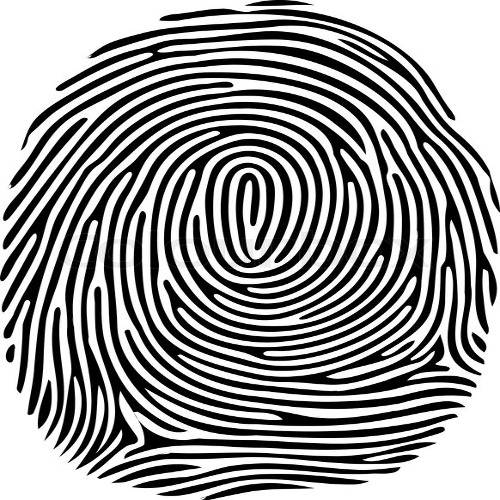
\includegraphics[width=0.325\linewidth]{./figures/experiments/fingerprint4.jpg}
    }
    \subfloat[][Computed Orientation field]{
	\label{fig:application_fingerprint1_noise}
	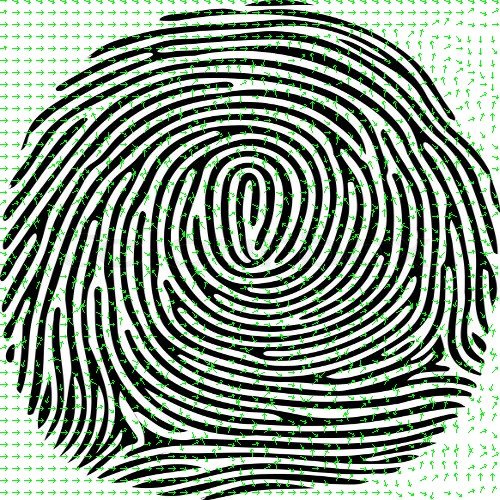
\includegraphics[width=0.325\linewidth]{./figures/experiments/input_fingerprint4.jpg}
    }
    \subfloat[][Denoised Orientation field]{
	\label{fig:application_fingerprint1_denoised}
	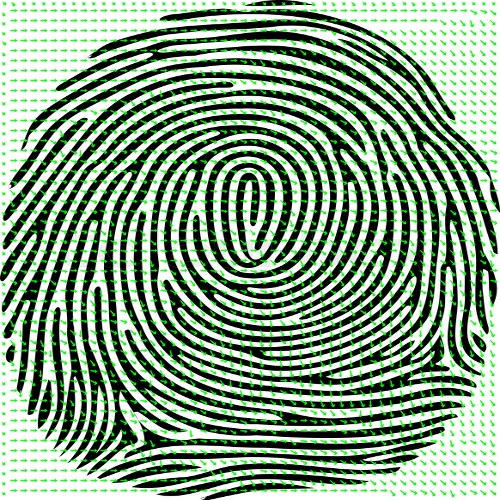
\includegraphics[width=0.325\linewidth]{./figures/experiments/denoised_fingerprint4.jpg}
    }\\
    \caption[Fingerprint orientation denoising]{Denoising a orientation field from a fingerprint, orientations represented by SO(2) elements
	\subref{fig:application_fingerprint1_orig} Original fingerprint 
	\subref{fig:application_fingerprint1_noise} Orientation field computed using Sobel derivatives PLACEHOLDER
	\subref{fig:application_fingerprint1_denoised} Denoised, IRLS with $\lambda=?$, $?$ IRLS steps, $?$ Newton steps per IRLS step PLACEHOLDER
	\label{fig:application_fingerprint1}
    }
\end{figure}

\FloatBarrier
\subsection{Reconstruction of a dense optical flow field} % (fold)
\label{sub:reconstructionDenseOpticalFlow}
An optical flow is the pattern of apparent motion between two consecutive frame of a video sequence. This may be the result of either an actual movement of the depicted object
or the result of a moving camera. Important applications are for example (anormal) motion detection, crowd behavior analysis, surveillance, video compression or image segmentation.\\
A \emph{dense} optical flow field can be interpreted as a vector field where each vector describes the displacement of a point between from one frame to the next. If
the set of points is retricted to only a few points of interest, a sparse feature set, we have \emph{sparse} optical flow.\\

In the following example, we only use a sparse feature set for tracking and flow computation in a short video sequence. The traffic scene was taken from a crowds/high density moving object data 
set provided by \cite{AliShah}. At first, we compute the sparse optical flow using the Lucas-Kanade algorithm \cite{LucasKanade} implemented in the OpenCV library. \\
For the set of tracked features 
$\mathcal{F}_1:=\lbrace{F^{(1)}_i\rbrace}_{i=1}^{400}\subset\Omega\subset\mathbb{R}^2$ in the first frame the algorithm tries to identify each feature in the second frame resulting in a set of
identified features $\mathcal{F}_2:=\lbrace{F^{(2)}_i\rbrace}_{i=1}^{N<400}\subset\Omega\subset\mathbb{R}^2$ and corresponding displacement vectors 
$\mathcal{V}_{12}:=\lbrace{V_i\,|\,V_i=F_i^{(2)}-F_i^{(1)}\rbrace}_{i=1}^{N}$.\\

We now assign to each pixel in our data an SO(2) element in the following way
\begin{align}
    \alpha_i &=\arctan\left(\frac{V^y_i}{V^x_i}\right) \\
    I(i,j) &= 
    \begin{cases}
    	\begin{pmatrix}
	    \cos\alpha_i    & -\sin\alpha_i\\
	    \sin\alpha_i    & \cos\alpha_i
	\end{pmatrix} & (i,j)\in \mathcal{F}_{2} \\
	0 & \text{ otherwise}
    \end{cases}
\end{align}

Since we want to reconstruct the dense flow, this is an inpainting problem and we have to perform scattered interpolation before running the algorithm. The result can be seen in 
Figure \ref{fig:application_flowfield1}.
\begin{figure}[h!]
    \centering
    \subfloat[][Original]{
	\label{fig:application_flowfield1_orig}
	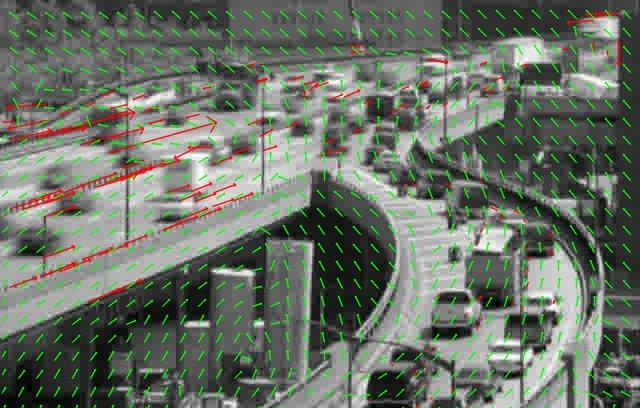
\includegraphics[width=0.325\linewidth]{./figures/experiments/reconstructed_optical_flow.jpg}
    }
    \subfloat[][Computed Sparse Flow field]{
	\label{fig:application_flowfield1_noise}
	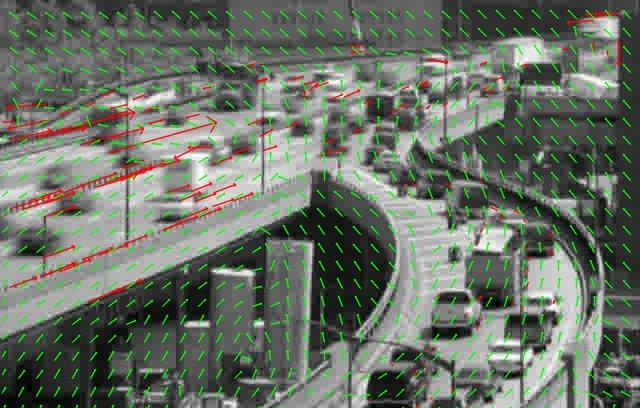
\includegraphics[width=0.325\linewidth]{./figures/experiments/reconstructed_optical_flow.jpg}
    }
    \subfloat[][Reconstructed orientation field]{
	\label{fig:application_flowfield1_denoised}
	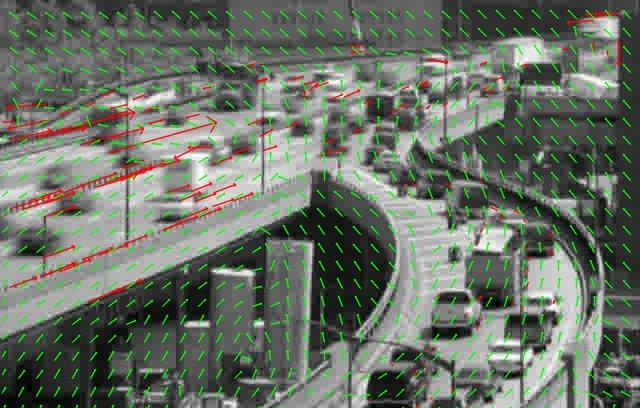
\includegraphics[width=0.325\linewidth]{./figures/experiments/reconstructed_optical_flow.jpg}
    }\\
    \caption[Dense optical flow reconstruction]{Reconstructing a dense flow from sparse feature tracking, orientations represented by SO(2) elements
	\subref{fig:application_flowfield1_orig} Frame of original video scene PLACEHOLDER
	\subref{fig:application_flowfield1_noise} Sparse features tracked using PLACEHOLDER
	\subref{fig:application_flowfield1_denoised} Reconstructed, IRLS with $\lambda=?$, $?$ IRLS steps, $?$ Newton steps per IRLS step
	\label{fig:application_flowfield1}
    }
\end{figure}

Of course the optimization could have also been performed on $S^1$. Furthermore, there is also a more direct, variational approach for the calculation of the flow field
which is also based on TV minimization but has a different fidelity term. This is one possibility for further extension of the library and is discussed in more detail in 
section \ref{sec:Extensions}

% subsection Calculation of a dense flow field (end)

% section SO(3) images data (end

\FloatBarrier
\section{SPD(3) image data} % (fold)
\label{sec:SPD(3) image data}

\subsection{Synthetic data} % (fold)
\label{sub:Synthetic data}

\begin{figure}[h!]
    \centering
    \subfloat[][Original]{
	\label{fig:application_spd1_orig}
	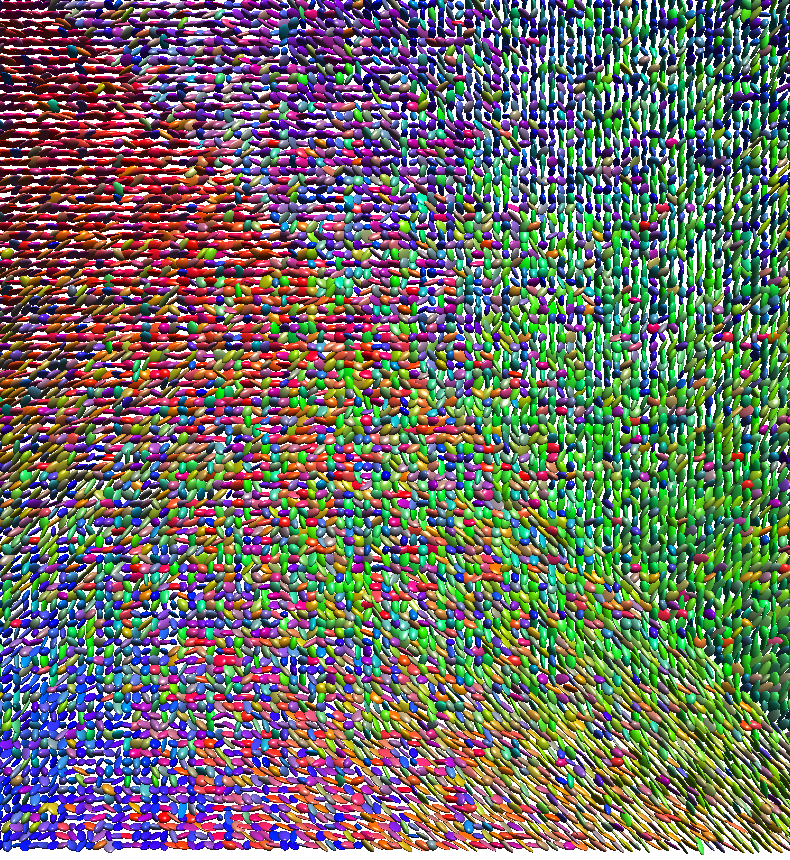
\includegraphics[width=0.325\linewidth]{./figures/experiments/noisy_spd100x100.png}
    }
    \subfloat[][Damaged]{
	\label{fig:application_spd1_noise}
	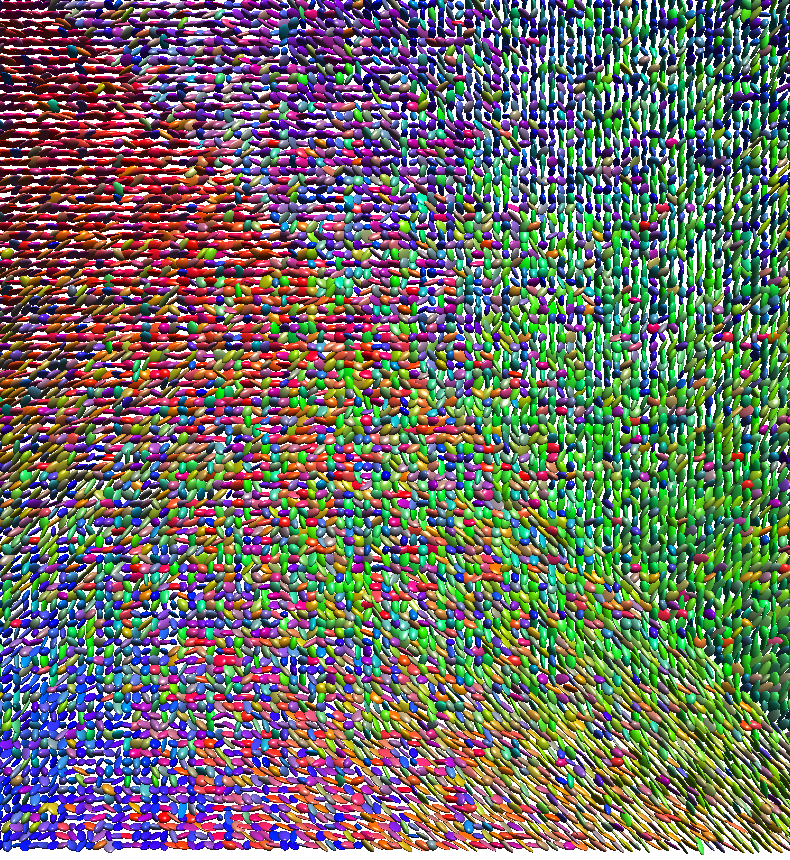
\includegraphics[width=0.325\linewidth]{./figures/experiments/noisy_spd100x100.png}
    }
    \subfloat[][Denoised]{
	\label{fig:application_spd1_denoised}
	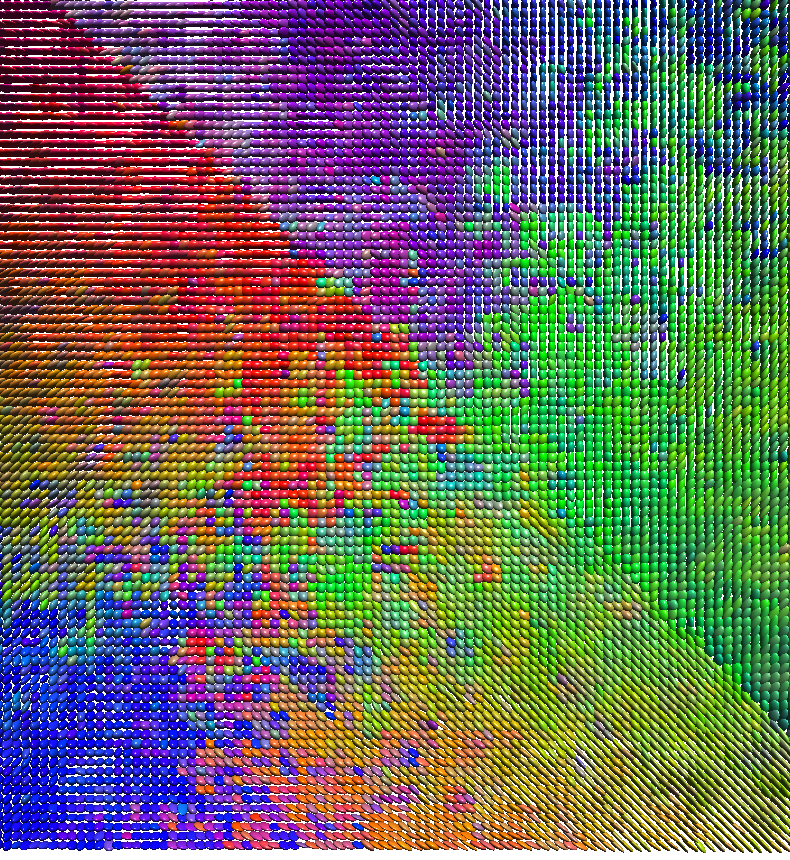
\includegraphics[width=0.325\linewidth]{./figures/experiments/denoised_spd100x100.png}
    }\\
    \caption[Denoising of synthetic SPD(3) picture]{Denoising of synthetic SPD(3) picture
	\subref{fig:application_spd1_orig} Original image: Synthetic, nonsmooth SPDO(3), $100\times 100$ px PLACEHOLDER
	\subref{fig:application_spd1_noise} Threshold $p=?$
	\subref{fig:application_spd1_denoised} Denoised, IRLS with $\lambda=?$, 5 IRLS steps, 1 Newton step per IRLS
	\label{fig:application_spd1}
    }
\end{figure}

% subsection Synthetic data (end)

\FloatBarrier
\subsection{Diffusion Tensor MRI images} % (fold)
\label{sub:Diffusion Tensor MRI images}
% subsection Diffusion Tensor MRI images (end)
\begin{figure}[h!]
    \centering
    \subfloat[][Noisy]{
	\label{fig:application_dti1_noise}
	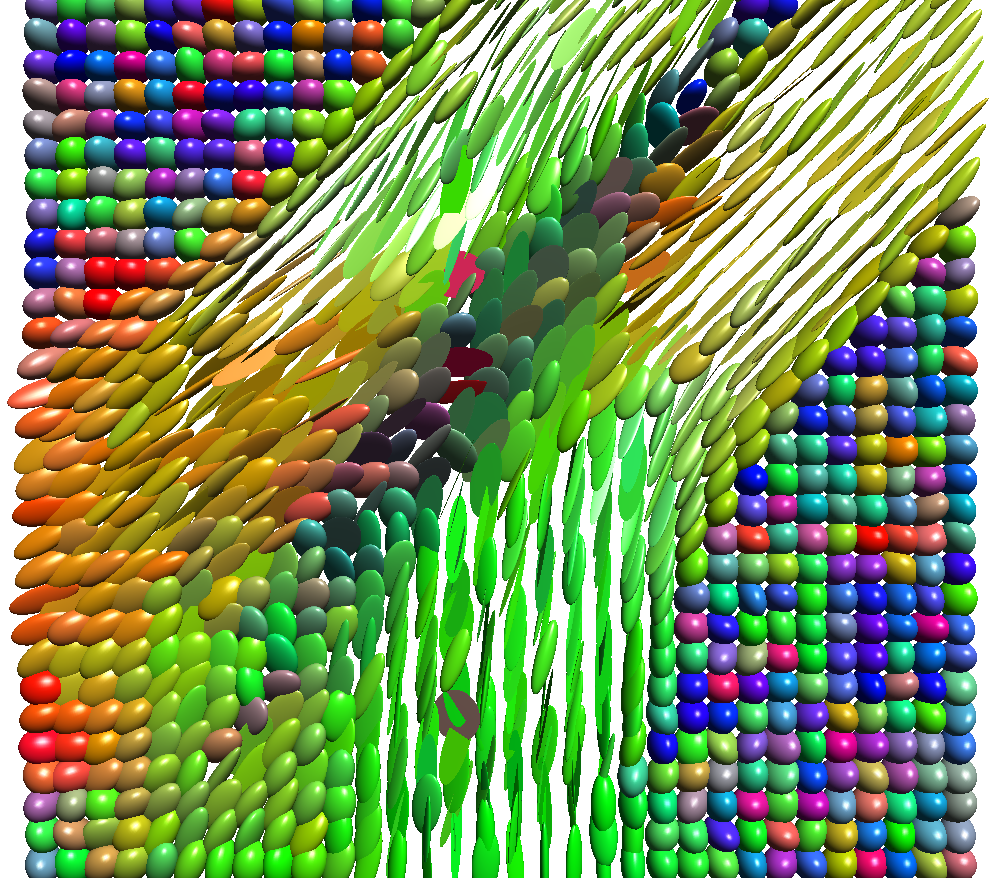
\includegraphics[width=0.5\linewidth]{./figures/experiments/noisy_dti32x32.png}
    }
    \subfloat[][Denoised]{
	\label{fig:application_dti1_denoised}
	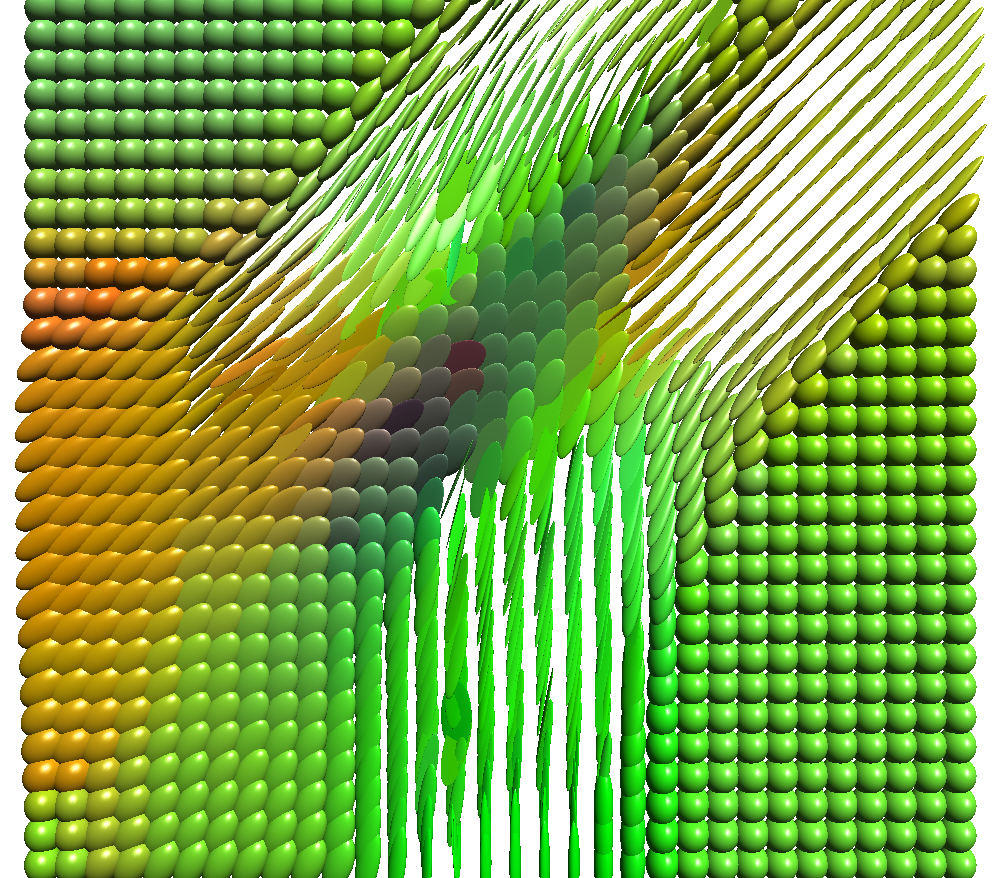
\includegraphics[width=0.5\linewidth]{./figures/experiments/denoised_dti32x32.png}
    }\\
    \caption[Denoising DT-MRI data]{Denoising a DT-MRI image with pixel in SPD(3)
	\subref{fig:application_dti1_noise} Componentwise gaussian noise $\mu=0$, $\sigma=?$ added
	\subref{fig:application_dti1_denoised} Denoised, IRLS with $\lambda=?$, $?$ IRLS steps, $?$ newton steps per IRLS step
	\label{fig:application_dti1}
    }
\end{figure}



\FloatBarrier
\subsection{3D DT MRI data} % (fold)
\label{sub:3DDTMRIdata}
% subsection 3D DT MRI data (end)
\begin{figure}[h!]
    \centering
    \subfloat[][Noisy]{
	\label{fig:application_dti2_noise}
	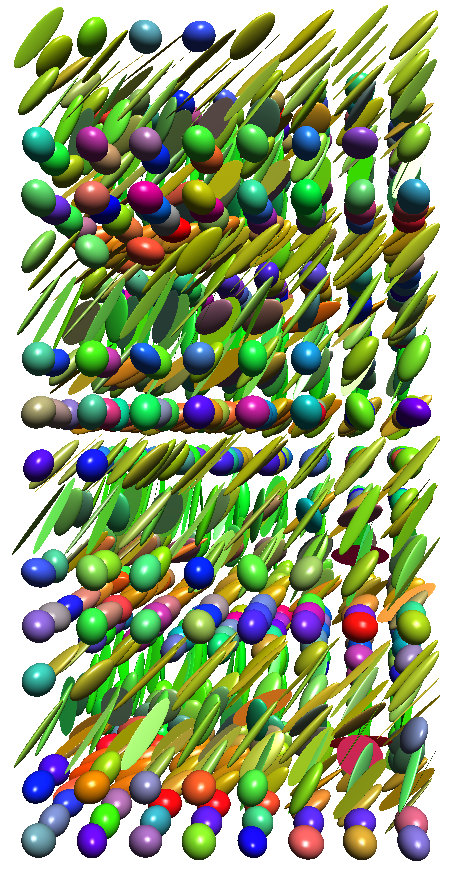
\includegraphics[width=0.4\linewidth]{./figures/experiments/noisy_dti3d8x16x16.png}
    }
    \subfloat[][Denoised]{
	\label{fig:application_dti2_denoised}
	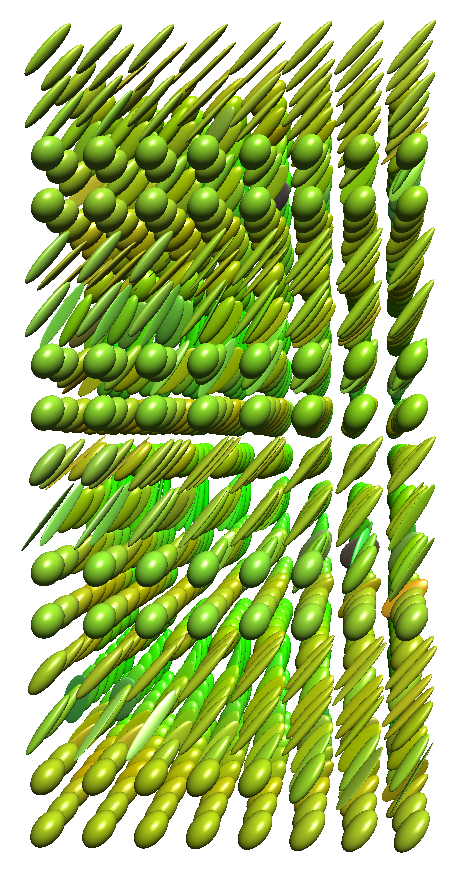
\includegraphics[width=0.4\linewidth]{./figures/experiments/denoised_dti3d8x16x16.png}
    }\\
    \caption[Denoising 3D DTI-MRI data]{Denoising a 3D DT-MRI image with pixel in SPD(3)
	\subref{fig:application_dti2_noise} Componentwise gaussian noise $\mu=0$, $\sigma=?$ added
	\subref{fig:application_dti2_denoised} Denoised, Proximal point with $\lambda=?$, 50 PRPT steps
	\label{fig:application_dti2}
    }
\end{figure}

% section SPD(3) image data (end)

\FloatBarrier
\section{Comparison IRLS and Proximal Point minimizers} % (fold)
\label{sec:Comparison IRLS and Proximal Point minimizers}

% section Comparison IRLS and Proximal Point minimizers (end)

\FloatBarrier
\section{Sensitivity to variations of the starting value} % (fold)
\label{sec:Sensitivity to variations of the starting value}

% section Sensitivity to variations of the starting value (end)

\end{chapter}
